\section{Gravitational wave detectors}

Ever since Michelson and Morley to designed an interferometer(IFO) to test Aether's existence \cite{Michelson333}, such device became widely used in several branches of physics where highly precise measurements were required. Applications of interferometry range from engineering and optics experiments to  quantum physics with the Mach-Zender IFO, and GW astronomy with the ground-based detectors GEO600, LIGO, Virgo and KAGRA.

The idea behind current ground based GW detectors keeps being as simple as the original design by Michelson and Morley(MM), but due to sensitivity requirements a lot of technological improvements have been implemented in order to mitigate noise sources like seismic noise, quatum shot noise and thermal noise \cite{LIGOScientific:2013pcc}. The picture below is taken from \cite{Hild_2012} and summarizes the main contributors to the advanced LIGO noise floor in the kHz band, also called \textit{sensitivity curve}  


\begin{figure}[hbt!]
\begin{center}
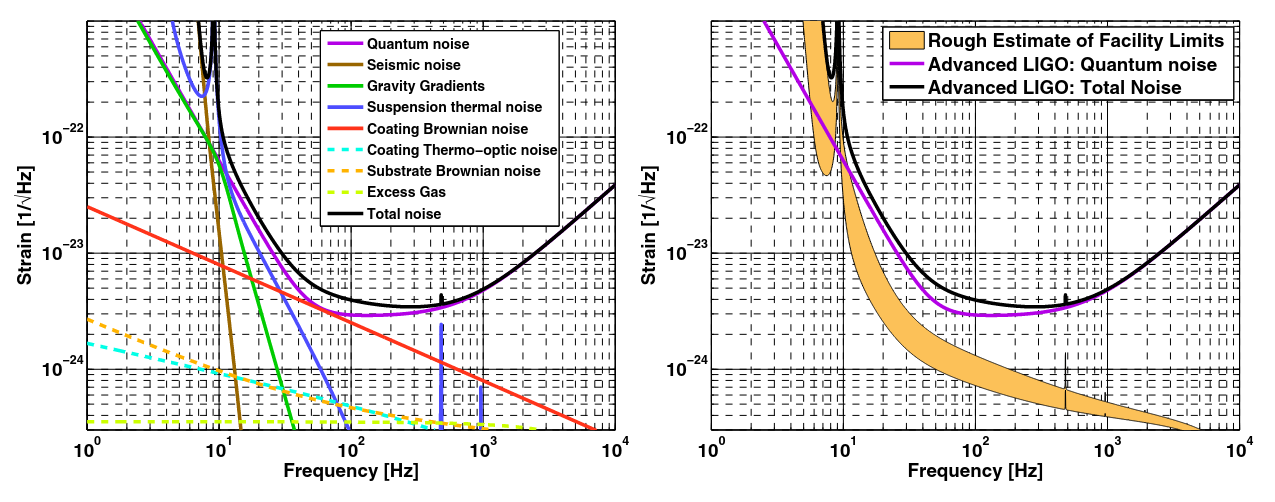
\includegraphics[width=0.7\textwidth, angle=0]{images/aligo.png}
\captionsetup{width=0.8\textwidth}
\caption{LIGO noise sources}
\caption*{This image was taken from \cite{Hild_2012}. It shows the noise floor of second-generation detectors, its decomposition on different noise sources, and their contribution to the amplitude spectral density of the detector(sensitivity curve).}
\label{LIGO}
\end{center}
\end{figure}
\FloatBarrier

In simple terms, the MM interferometers are composed by: a very stable laser, a reflective mirror called beam splitter(BS) and two perpendicular arms with mirrors at their ends, called Fabry-Perrot cavities \cite{Saulson:1995zi}. The following figure taken from \cite{Hild_2012} shows the simplified schematics of an L shaped IFO   


\begin{figure}[hbt!]
\begin{center}
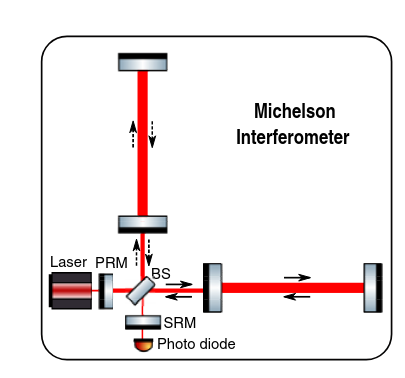
\includegraphics[width=0.35\textwidth, angle=0]{images/IFO.png}
\captionsetup{width=0.8\textwidth}
\caption{Simplified L-shaped interferometer}
\label{IFO}
\end{center}
\end{figure}

\FloatBarrier

The laser passes through the BS and gets decomposed in 2 perpendicular beams such that after each roundtrip recombine at the IFO output where a photodiode is located. The IFO is sensitive to proper lenght changes in the fabry-perrot cavities caused by a GW interacting with its test masses(endmirrors). Consequently, the photodiode measures power variations at the IFO output, caused by changes in the beam roundtrip time, that translate into phase differences when both perpendicular beams recombine.

To see that, consider the arm pointing in the horizontal direction in figure \ref{IFO}, and a gravitational wave with only $h_+$  polarization traveling in the z-direction perpendicular to the detector plane. The line element \ref{GWlineelement} in the TT gauge is given by

\begin{equation}
ds^2 = c^2 dt^2 - (1-h_+) dx^2 - (1+h+) dy^2 + dz^2
\end{equation}

Given that photons travel in null geodesics $ds^2 = 0$, the distance traveled in the x direction by the light beam is given by

\begin{equation}\label{dx}
dx \approx \pm cdt \left(  1-\frac{1}{2} h_+ \right)
\end{equation}

Where we used the first order approximation $(1+x)^{-\frac{1}{2}} \approx (1 - \frac{1}{2} x)$. The plus sign can be associated with the travel from the beam splitter to the mirror and the minus with the return trip. 

Let us define the starting time where the beam leaves the beamsplitter $t_0$, the time $t_1$ where the beam reaches the mirror, and the time $t_2$ when the beam returns to the beam splitter(see Maggiore \cite[chapter 9]{Maggiore:2007ulw}). The distances traveled in the plus and minus directions can be computed by integrating \ref{dx}

\begin{equation}
L_{x}  = \int_0^{L_x} dx = \int_{t_0}^{t_1} dt' \left[+c \cdot\left(1-\frac{1}{2} h_+(t') \right)\right] = c\cdot(t_1-t_0) - \frac{c}{2} \int_{t_0}^{t_1} dt' h_+(t') 
\end{equation}

\begin{equation}
-L_{x}  = \int^0_{L_x} dx = \int_{t_1}^{t_2} dt' \left[-c \cdot\left(1-\frac{1}{2} h_+(t') \right)\right] = c\cdot(t_1-t_2) - \frac{c}{2} \int_{t_1}^{t_2} dt' h_+(t')
\end{equation}


Which can then be summed to eliminate $t_1$ and get the round trip time $t_2-t_0$.

\begin{equation}
2L_x = c(t_2 - t_0) + \frac{c}{2} \left[ \int_{t_0}^{t_1} dt' h_+(t') +  \int_{t_1}^{t_2} dt' h_+(t')\right]
\end{equation}

\begin{equation}
t_2 - t_0 = \frac{2L_x}{c} + \frac{1}{2} \int_{t_0}^{t_2} dt' h_+(t')
\end{equation}

Similarly for the arm in the y-direction we get

\begin{equation}
t_2 - t_0 = \frac{2L_y}{c} - \frac{1}{2} \int_{t_0}^{t_2} dt' h_+(t')
\end{equation}

One can clearly see that the round trip time of the beam $\frac{2L_x}{c}$ is modified by $\delta \tau_{rt} = \frac{1}{2} \int_{t_0}^{t_2} dt' h_+(t')$. The round trip time variations caused by the gravitational wave can be further shown to affect the phases of the beams and then make possible its detection from power fluctuations at the photodiode readout \cite{Saulson:1995zi}. The round trip phase changes caused by the interaction of the GW with the IFO arms, can be computed using 

\begin{equation}
x-direction \rightarrow \delta \phi_{rt} = k\cdot c \cdot \delta \tau_{rt}
\end{equation}

\begin{equation}
y-direction \rightarrow \delta \phi*_{rt} = - k\cdot c \cdot \delta \tau_{rt}
\end{equation}
